\let\negmedspace\undefined
\let\negthickspace\undefined
\documentclass[journal,12pt,onecolumn]{IEEEtran}
\usepackage{cite}
\usepackage{amsmath,amssymb,amsfonts,amsthm}
\usepackage{algorithmic}
\usepackage{graphicx}
\usepackage{textcomp}
\usepackage{xcolor}
\usepackage{txfonts}
\usepackage{listings}
\usepackage{enumitem}
\usepackage{mathtools}
\usepackage{gensymb}
\usepackage[breaklinks=true]{hyperref}
\usepackage{tkz-euclide} % loads  TikZ and tkz-base
\usepackage{listings}
\usepackage{float}



\newtheorem{theorem}{Theorem}[section]
\newtheorem{problem}{Problem}
\newtheorem{proposition}{Proposition}[section]
\newtheorem{lemma}{Lemma}[section]
\newtheorem{corollary}[theorem]{Corollary}
\newtheorem{example}{Example}[section]
\newtheorem{definition}[problem]{Definition}
%\newtheorem{thm}{Theorem}[section] 
%\newtheorem{defn}[thm]{Definition}
%\newtheorem{algorithm}{Algorithm}[section]
%\newtheorem{cor}{Corollary}
\newcommand{\BEQA}{\begin{eqnarray}}
\newcommand{\EEQA}{\end{eqnarray}}
\newcommand{\define}{\stackrel{\triangle}{=}}
\theoremstyle{remark}
\newtheorem{rem}{Remark}
%\bibliographystyle{ieeetr}
\begin{document}
%
\providecommand{\pr}[1]{\ensuremath{\Pr\left(#1\right)}}
\providecommand{\prt}[2]{\ensuremath{p_{#1}^{\left(#2\right)} }}        % own macro for this question
\providecommand{\qfunc}[1]{\ensuremath{Q\left(#1\right)}}
\providecommand{\sbrak}[1]{\ensuremath{{}\left[#1\right]}}
\providecommand{\lsbrak}[1]{\ensuremath{{}\left[#1\right.}}
\providecommand{\rsbrak}[1]{\ensuremath{{}\left.#1\right]}}
\providecommand{\brak}[1]{\ensuremath{\left(#1\right)}}
\providecommand{\lbrak}[1]{\ensuremath{\left(#1\right.}}
\providecommand{\rbrak}[1]{\ensuremath{\left.#1\right)}}
\providecommand{\cbrak}[1]{\ensuremath{\left\{#1\right\}}}
\providecommand{\lcbrak}[1]{\ensuremath{\left\{#1\right.}}
\providecommand{\rcbrak}[1]{\ensuremath{\left.#1\right\}}}
\newcommand{\sgn}{\mathop{\mathrm{sgn}}}
\providecommand{\abs}[1]{\left\vert#1\right\vert}
\providecommand{\res}[1]{\Res\displaylimits_{#1}} 
\providecommand{\norm}[1]{\left\lVert#1\right\rVert}
%\providecommand{\norm}[1]{\lVert#1\rVert}
\providecommand{\mtx}[1]{\mathbf{#1}}
\providecommand{\mean}[1]{E\left[ #1 \right]}
\providecommand{\cond}[2]{#1\middle|#2}
\providecommand{\fourier}{\overset{\mathcal{F}}{ \rightleftharpoons}}
\newenvironment{amatrix}[1]{%
  \left(\begin{array}{@{}*{#1}{c}|c@{}}
}{%
  \end{array}\right)
}
%\providecommand{\hilbert}{\overset{\mathcal{H}}{ \rightleftharpoons}}
%\providecommand{\system}{\overset{\mathcal{H}}{ \longleftrightarrow}}
	%\newcommand{\solution}[2]{\textbf{Solution:}{#1}}
\newcommand{\solution}{\noindent \textbf{Solution: }}
\newcommand{\cosec}{\,\text{cosec}\,}
\providecommand{\dec}[2]{\ensuremath{\overset{#1}{\underset{#2}{\gtrless}}}}
\newcommand{\myvec}[1]{\ensuremath{\begin{pmatrix}#1\end{pmatrix}}}
\newcommand{\mydet}[1]{\ensuremath{\begin{vmatrix}#1\end{vmatrix}}}
\newcommand{\myaugvec}[2]{\ensuremath{\begin{amatrix}{#1}#2\end{amatrix}}}
\providecommand{\rank}{\text{rank}}
\providecommand{\pr}[1]{\ensuremath{\Pr\left(#1\right)}}
\providecommand{\qfunc}[1]{\ensuremath{Q\left(#1\right)}}
	\newcommand*{\permcomb}[4][0mu]{{{}^{#3}\mkern#1#2_{#4}}}
\newcommand*{\perm}[1][-3mu]{\permcomb[#1]{P}}
\newcommand*{\comb}[1][-1mu]{\permcomb[#1]{C}}
\providecommand{\qfunc}[1]{\ensuremath{Q\left(#1\right)}}
\providecommand{\gauss}[2]{\mathcal{N}\ensuremath{\left(#1,#2\right)}}
\providecommand{\diff}[2]{\ensuremath{\frac{d{#1}}{d{#2}}}}
\providecommand{\myceil}[1]{\left \lceil #1 \right \rceil }
\newcommand\figref{Fig.~\ref}
\newcommand{\systemL}[1]{\stackrel{#1}{\xleftrightarrow{\mathcal{L}}}}
\newcommand{\systemLinv}[1]{\stackrel{#1}{\xleftrightarrow{\mathcal{L}^{-1}}}}


\newcommand\tabref{Table~\ref}
\newcommand{\sinc}{\,\text{sinc}\,}
\newcommand{\rect}{\,\text{rect}\,}
%%
%	%\newcommand{\solution}[2]{\textbf{Solution:}{#1}}
%\newcommand{\solution}{\noindent \textbf{Solution: }}
%\newcommand{\cosec}{\,\text{cosec}\,}
%\numberwithin{equation}{section}
%\numberwithin{equation}{subsection}
%\numberwithin{problem}{section}
%\numberwithin{definition}{section}
%\makeatletter
%\@addtoreset{figure}{problem}
%\makeatother

%\let\StandardTheFigure\thefigure
\let\vec\mathbf


\bibliographystyle{IEEEtran}
\title{ EE1204 ASSIGNMENT-1}
\author{EE23BTECH11011- BATCHU ISHITHA \\ EE23BTECH11061- SWATHI$^{*}$% <-this % stops a space
}

\maketitle




\bigskip

\renewcommand{\thefigure}{\theenumi}
\renewcommand{\thetable}{\theenumi}
%\renewcommand{\theequation}{\theenumi}
\textbf{SOFTWARE USED}:\\ MATHEMATICA FOR QUESTION 1 AND 2; SIM SCALE FOR QUESTION 3.\\

1: A field is given in spherical co-ordinates: $[5 points]$ 
$$\overrightarrow{F}=\frac{1}{r^2}\cos \phi \mathrm{\hat{r}} + \frac{\sin \phi}{r^2 \sin \theta} \mathrm{\hat{\phi}}$$ 
(1.1) Plot (a)$\abs{\overrightarrow{F}}$ vs $\phi$ for $r=0.8$ (b)  $\abs{\overrightarrow{F}}$ vs $r$ for $\phi = 45\degree$ \\
(1.2) Calculate with computer , verify with hand calculations (a)$\overrightarrow{\nabla}.\overrightarrow{F}$ (b)$\overrightarrow{\nabla}X\overrightarrow{F} $ (c)$\overrightarrow{\nabla}\brak{\overrightarrow{\nabla}.\overrightarrow{F}}$ \\
(1.3) Check if $\overrightarrow{F}$ is a valid electrostatic field using two methods. \\

\solution \\
(1.1)(a)
\begin{figure}[H]
    \centering
     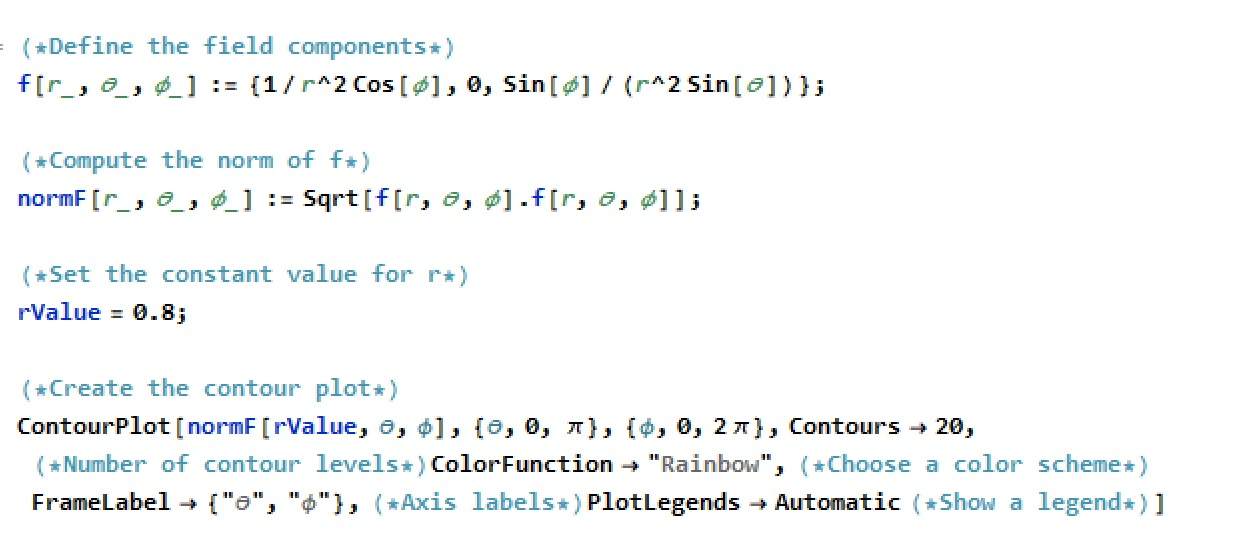
\includegraphics[scale=0.5]{figs/1.1.1.jpeg}
    \caption{}    
    \label{fig:ishitha.em.fig1}
\end{figure}
\begin{figure}[H]
    \centering
     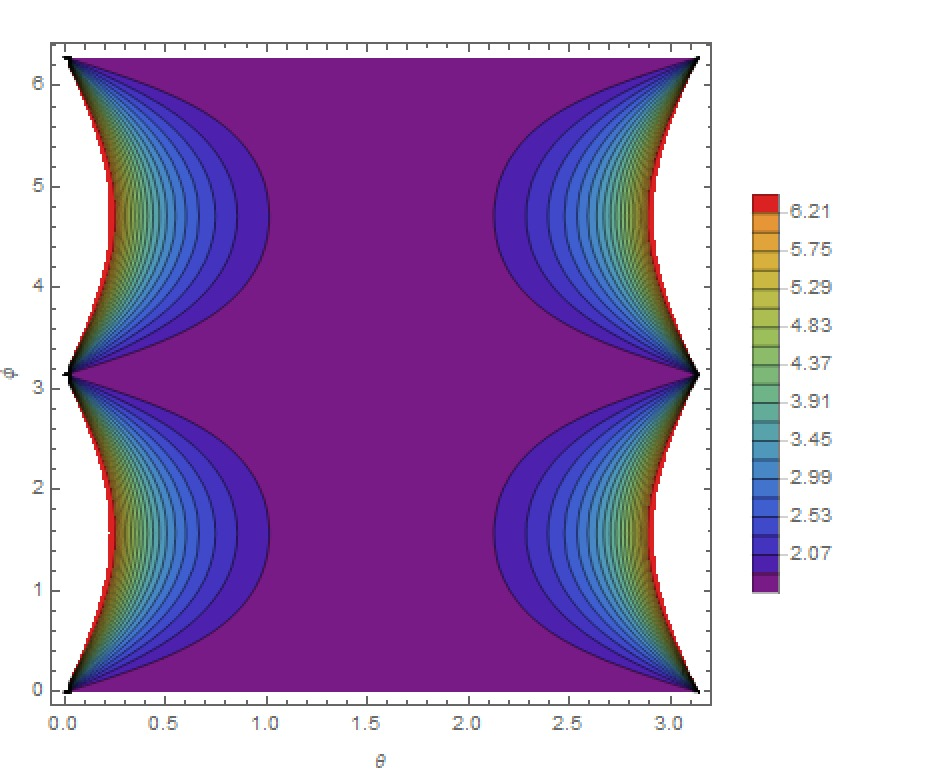
\includegraphics[scale=0.5]{figs/1.1.2.jpeg}
    \caption{}    
    \label{fig:ishitha.em.fig1}
\end{figure}

(b)
\begin{figure}[H]
    \centering
     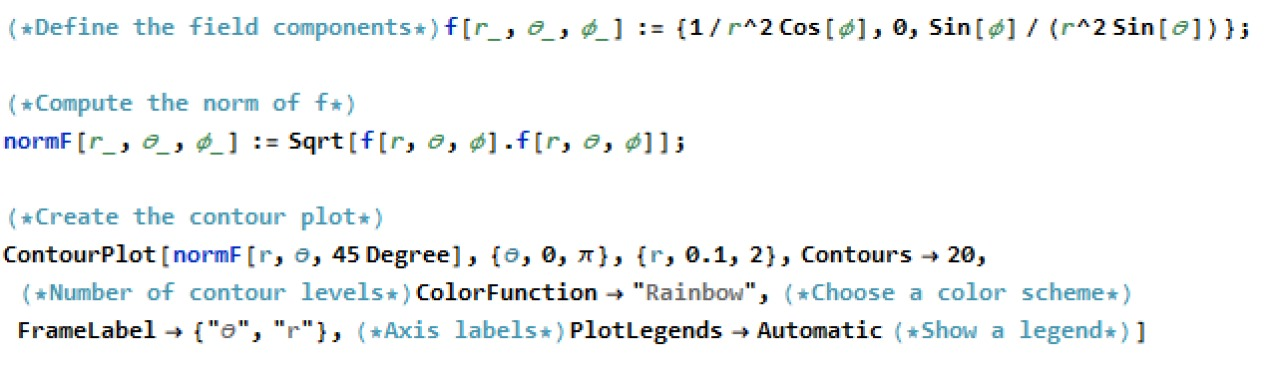
\includegraphics[scale=0.5]{figs/1.2.1.jpeg}
    \caption{}    
    \label{fig:ishitha.em.fig1}
\end{figure}
\begin{figure}[H]
    \centering
     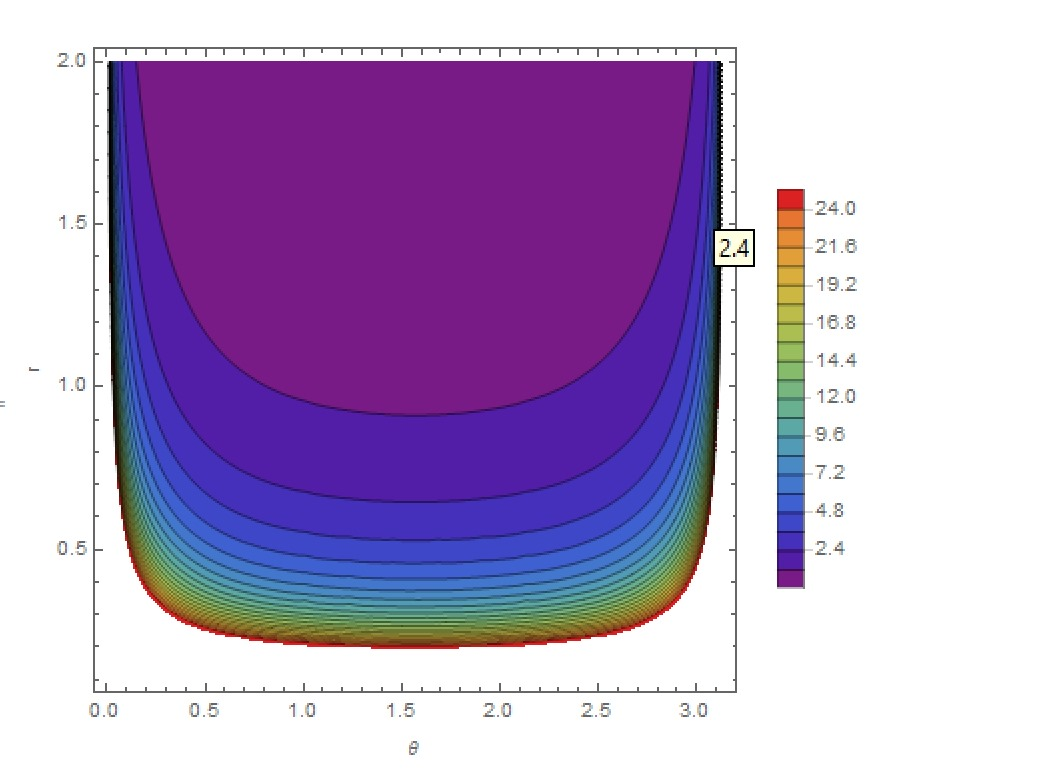
\includegraphics[scale=0.5]{figs/1.2.2.jpeg}
    \caption{}    
    \label{fig:ishitha.em.fig1}
\end{figure}
(1.2) (a) \begin{figure}[H]
    \centering
     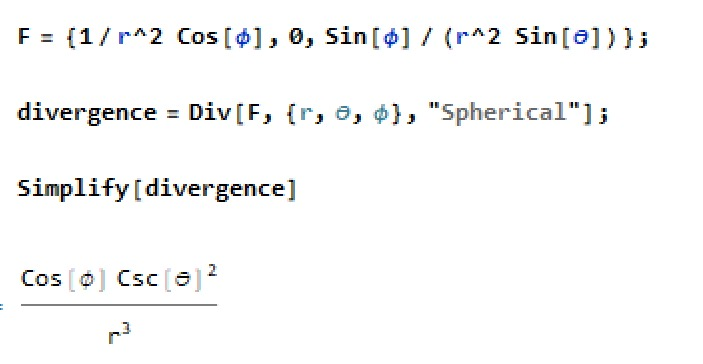
\includegraphics[scale=0.5]{figs/div.jpeg}
    \caption{}    
    \label{fig:ishitha.em.fig1}
\end{figure}
 (a) HAND CALCULATION:\\
\begin{align}
\overrightarrow{\nabla}.\overrightarrow{F}&=\brak{\frac{1}{r^2}\frac{\partial r^2}{\partial  r}\hat{r}+\frac{1}{r\sin\theta }\frac{\partial \sin\theta }{\partial \theta}\hat{\theta}+\frac{1}{r\sin\theta}\frac{\partial }{\partial \phi}\hat{\phi}}.\brak{\frac{1}{r^2}\cos \phi \hat{r} + \frac{\sin \phi}{r^2 \sin \theta} \hat{\phi}}\\
&= \frac{1}{r^2}\frac{\partial \brak{r^2\frac{\cos\phi}{r^2}}}{\partial  r}+\frac{1}{r\sin\theta }\frac{\partial \sin\theta(0)}{\partial \theta} +\frac{1}{r\sin\theta}\frac{\partial \brak{\frac{\sin\phi}{r^2\sin\theta}}}{\partial \phi}\\
&=0+0+\frac{\cos\phi}{r^3\sin^2\theta}\\
\implies \overrightarrow{\nabla}.\overrightarrow{F}&=\frac{\cos\phi}{r^3\sin^2\theta}
\end{align}

(b)  \begin{figure}[H]
    \centering
     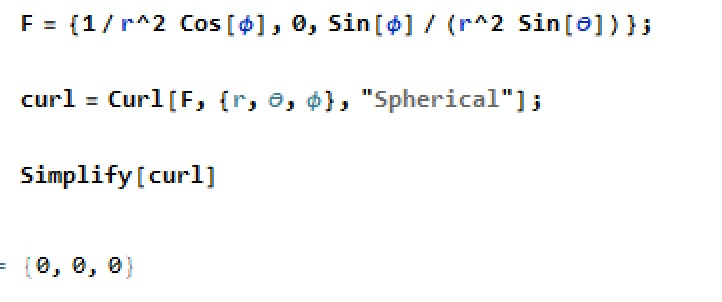
\includegraphics[scale=0.5]{figs/curl.jpeg}
    \caption{}    
    \label{fig:ishitha.em.fig1}
\end{figure}
HAND CALCULATION:\\
\begin{align}
\overrightarrow{\nabla}X\overrightarrow{F}&=
\frac{1}{r^2\sin\theta}det\myvec{
\hat{r} & r\hat{\theta} & r\sin\theta\hat{\phi} \\
\frac{\partial}{\partial r}&\frac{\partial}{\partial \theta}&\frac{\partial}{\partial\phi}\\
\frac{1}{r^2}\cos \phi &r.0&r\sin\theta\frac{\sin \phi}{r^2 \sin \theta}
}
\end{align}

\begin{align}
&=\frac{1}{r^2\sin\theta}\sbrak{\hat{r}\brak{\frac{\partial\brak{\frac{\sin\phi}{r}}}{\partial \theta}-\frac{\partial (0)}{\partial \phi}}-r \hat{\theta}\brak{\frac{\partial\brak{\frac{\sin\phi}{r}}}{\partial r}-\frac{\partial \brak{\frac{\cos\phi}{r^2}}}{\partial \phi}}+r \sin\theta\hat{\phi}\brak{\frac{\partial (0)}{\partial r} -\frac{\partial\brak{\frac{\cos\phi}{r^2}}}{\partial \theta}}} \\
&={r^2\sin\theta}\sbrak{(0-0)\hat{r}-\brak{\frac{-\sin\phi}{r^2}-\frac{-\sin\phi}{r^2}}r\hat{\theta}+(0-0)r\sin\theta\hat{\phi}}\\
&=0\hat{r}+0\hat{\theta}+0\hat{\phi}
\end{align}


(c)\begin{figure}[H]
    \centering
     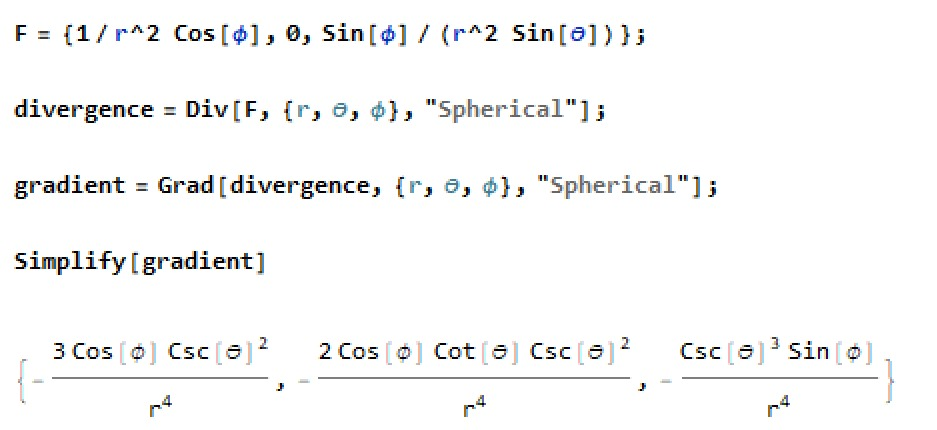
\includegraphics[scale=0.5]{figs/grad(div).jpeg}
    \caption{}    
    \label{fig:ishitha.em.fig1}
\end{figure} 
HAND CALCULATION:\\
\begin{align}
\overrightarrow{\nabla}\brak{\overrightarrow{\nabla}.\overrightarrow{F}}&=\overrightarrow{\nabla}\brak{\frac{\cos\phi}{r^3\sin^2\theta}}\\
&=\brak{\frac{\partial}{\partial r}\hat{r}+\frac{1}{r }\frac{\partial}{\partial \theta}\hat{\theta}+\frac{1}{r\sin\theta}\frac{\partial}{\partial \phi}\hat{\phi}}\brak{\frac{\cos \phi}{r^3 \sin^2 \theta}}\\
&= \brak{\frac{-3\cos \phi}{r^4\sin^2\theta}}\hat{r}-\brak{\frac{2\cos \phi \cot \theta}{r^4 \sin^2 \theta}}\hat{\theta}+\brak{-\frac{\sin \phi}{r^4 \sin^3 \theta}}\hat{\phi}
\end{align}

(1.3)\\ 
METHOD-1: CURL OF $\overrightarrow{F}$:\\
If the curl of the electrostatic field is zero, it indicates that electrostatic field is conservative,\\
 ie: $\overrightarrow{F}$ is a valid electrostatic field.
 
\begin{align}
\overrightarrow{\nabla}X\overrightarrow{F}&=
\frac{1}{r^2\sin\theta}det\myvec{
\hat{r} & r\hat{\theta} & r\sin\theta\hat{\phi} \\
\frac{\partial}{\partial r}&\frac{\partial}{\partial \theta}&\frac{\partial}{\partial\phi}\\
\frac{1}{r^2}\cos \phi &r.0&r\sin\theta\frac{\sin \phi}{r^2 \sin \theta}
}
\end{align}

\begin{align}
&=\frac{1}{r^2\sin\theta}\sbrak{\hat{r}\brak{\frac{\partial\brak{\frac{\sin\phi}{r}}}{\partial \theta}-\frac{\partial (0)}{\partial \phi}}-r \hat{\theta}\brak{\frac{\partial\brak{\frac{\sin\phi}{r}}}{\partial r}-\frac{\partial \brak{\frac{\cos\phi}{r^2}}}{\partial \phi}}+r \sin\theta\hat{\phi}\brak{\frac{\partial (0)}{\partial r} -\frac{\partial\brak{\frac{\cos\phi}{r^2}}}{\partial \theta}}} \\
&={r^2\sin\theta}\sbrak{(0-0)\hat{r}-\brak{\frac{-\sin\phi}{r^2}-\frac{-\sin\phi}{r^2}}r\hat{\theta}+(0-0)r\sin\theta\hat{\phi}}\\
&=0\hat{r}+0\hat{\theta}+0\hat{\phi}
\end{align}
Therefore,  $\overrightarrow{F}$ is a valid electrostatic field.\\
METHOD-2:STOKE'S THEOREM:\\
\[
\iint_S (\nabla X \overrightarrow{F}) \cdot d\mathbf{a} = \oint_C \overrightarrow{F} \cdot d\mathbf{l}
\]
From the above equation , since curl of $\overrightarrow{F}$ is zero,it is conservative in nature,ie: it is a valid electrostatic field.\\


2: Consider the charge configuration :$[5 points]$ \\
\begin{figure}[H]
    \centering
     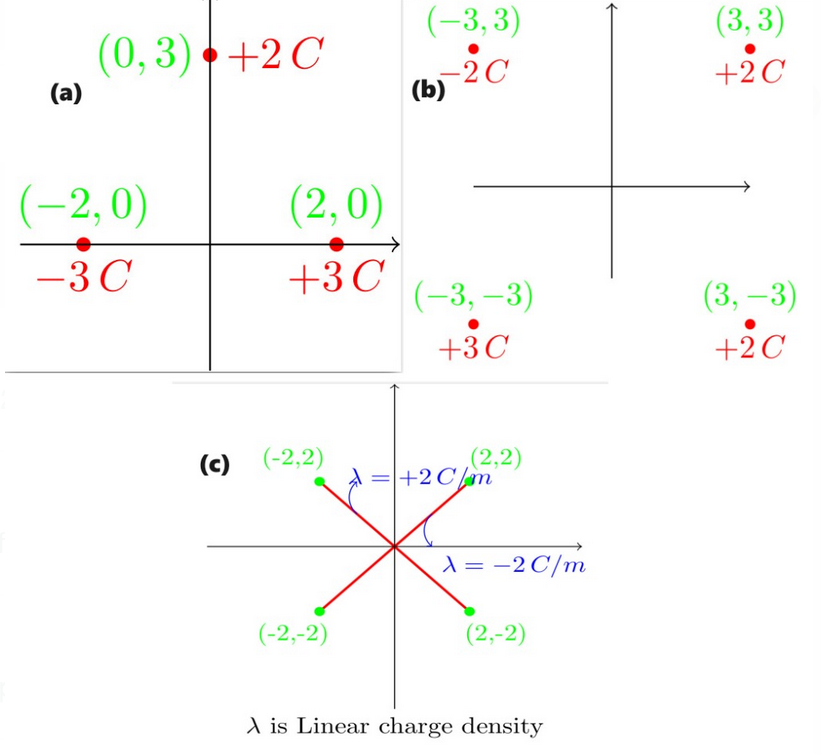
\includegraphics[scale=0.20]{figs/fig1.png}
    \caption{}    
    \label{fig:ishitha.em.fig1}
\end{figure}
(2.1) Plot for all the charge configurations for $(x,y)=(\pm 6,\pm 6)$ (a) $\overrightarrow{E}$ (b) V (c) U(Electrostatic Energy)\\
(2.2) Verify through graphical visualisation/representation (a) GAUSS'S LAW (b)$\overrightarrow{E}=\nabla{V}$ \\(c) $\overrightarrow{E}$ is conservative \\
(2.3) Calculate the force acting on unit charge sitting in origin due to charge configurations.\\

\solution \\
(2.1.(a))\\
(a)
\begin{figure}[H]
    \centering
     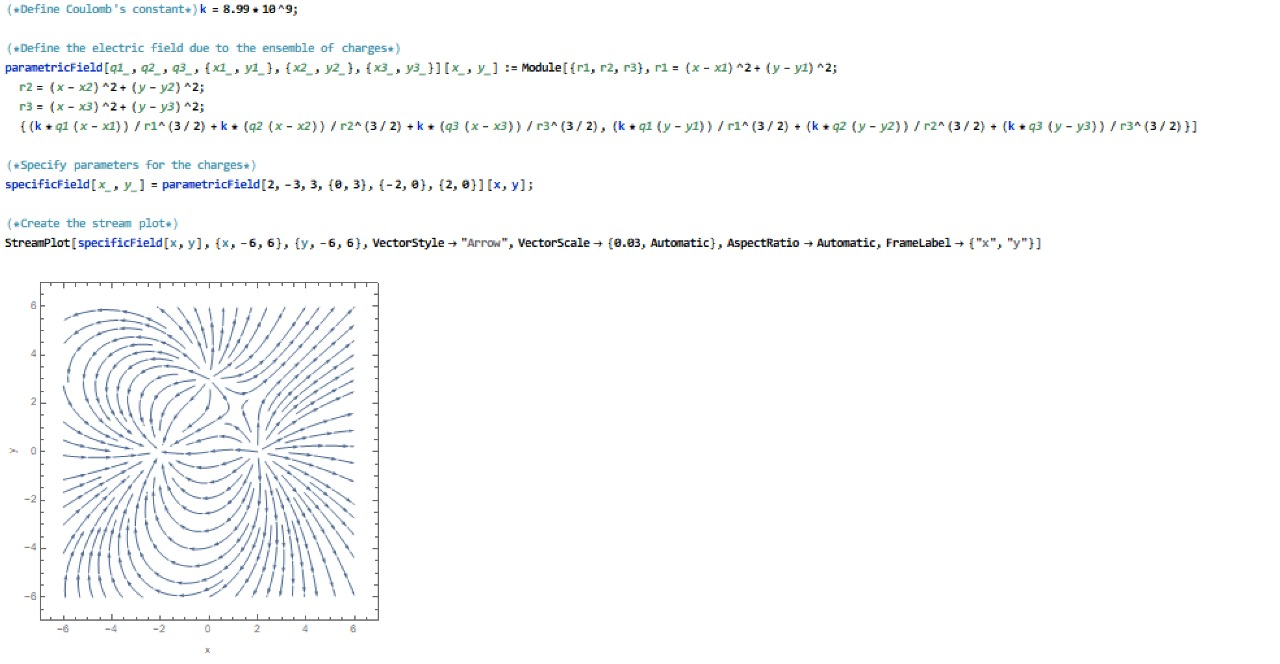
\includegraphics[scale=0.40]{figs/e1.jpeg}
    \caption{}    
    \label{fig:ishitha.em.fig1}
\end{figure}

(b)\begin{figure}[H]
    \centering
     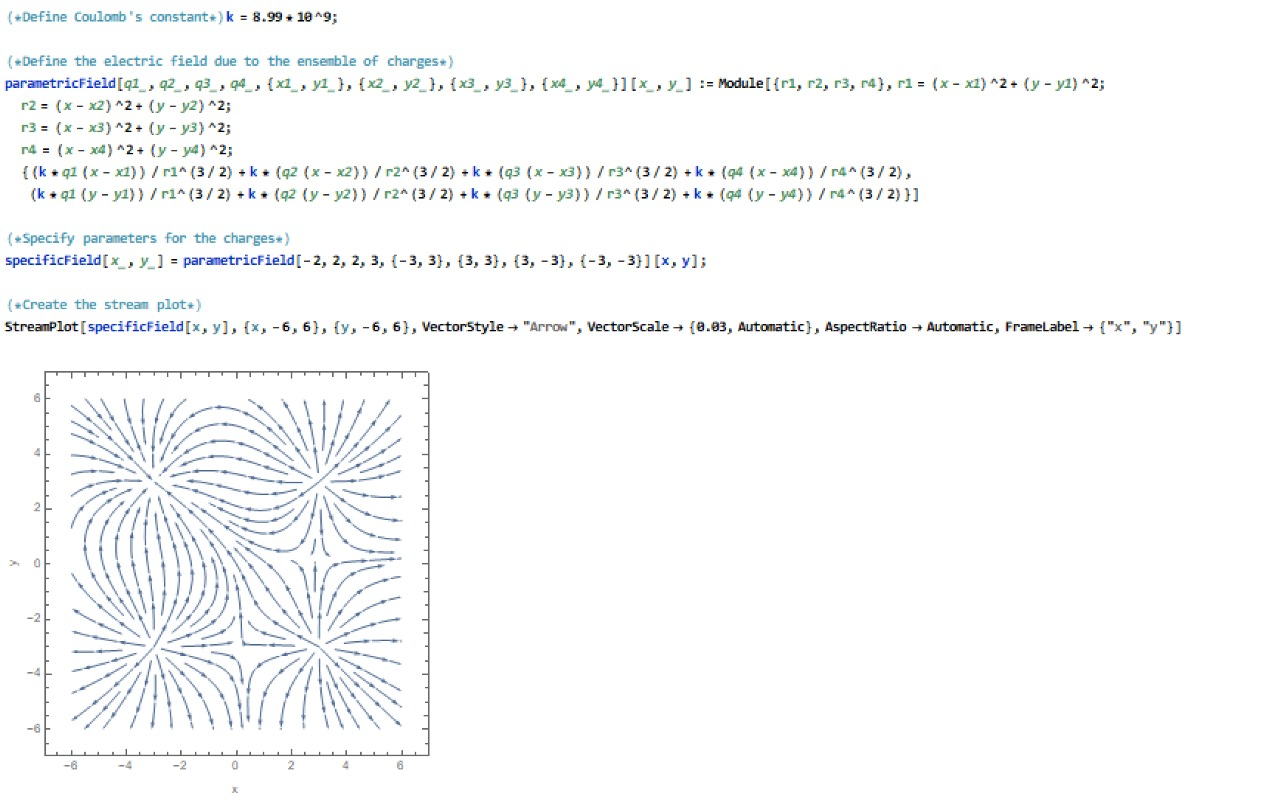
\includegraphics[scale=0.4]{figs/e2.jpeg}
    \caption{}    
    \label{fig:ishitha.em.fig1}
\end{figure}
\newpage
(c)\\
\begin{figure}[H]
    \centering
     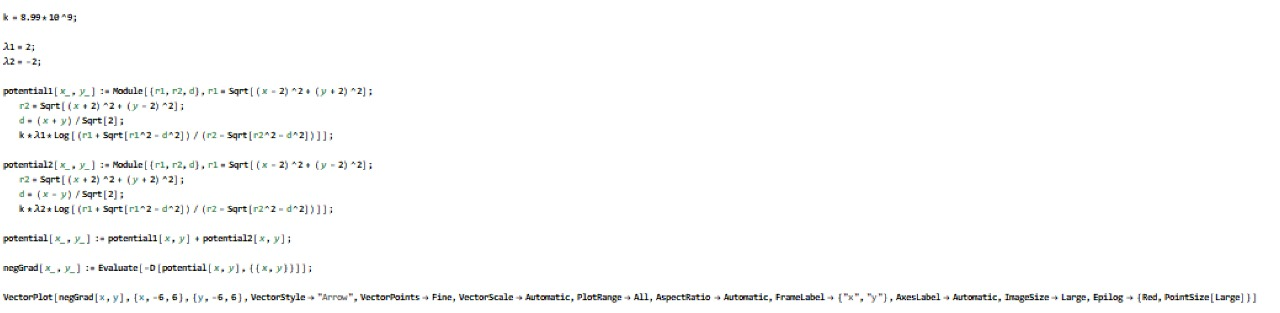
\includegraphics[scale=0.55]{figs/e.1.1.jpeg}
    \caption{}    
    \label{fig:ishitha.em.fig1}
   \end{figure} \begin{figure}[H]
    \centering
     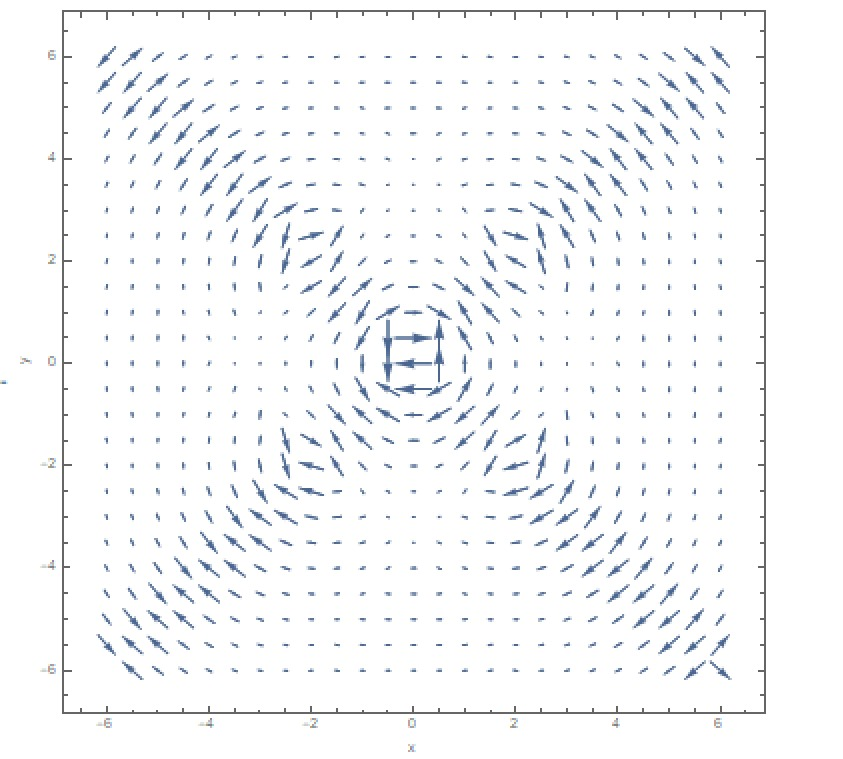
\includegraphics[scale=0.5]{figs/e.1.jpeg}
    \caption{}    
    \label{fig:ishitha.em.fig1}
   \end{figure}
   \newpage
(2.1.(b))\\
(a)
\begin{figure}[H]
    \centering
     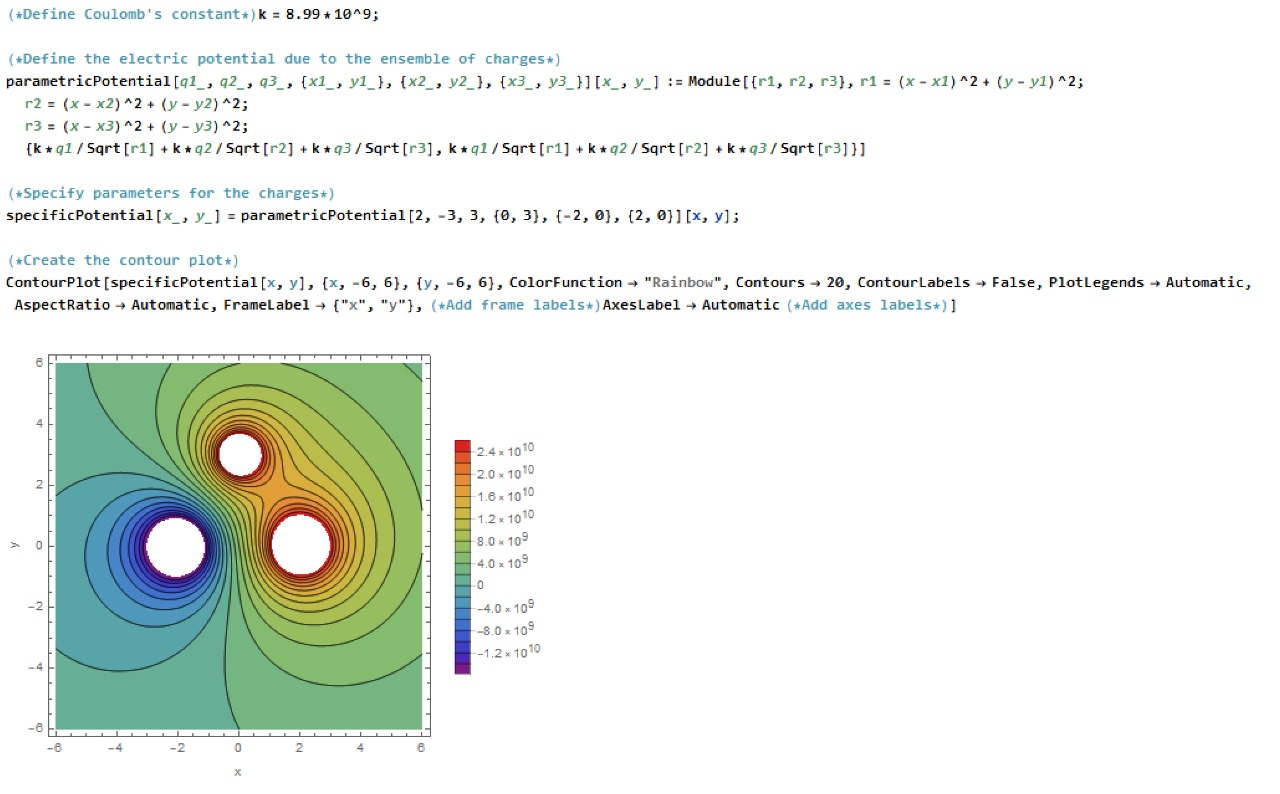
\includegraphics[scale=0.40]{figs/v1.jpeg}
    \caption{}    
    \label{fig:ishitha.em.fig1}
\end{figure}

(b)\begin{figure}[H]
    \centering
     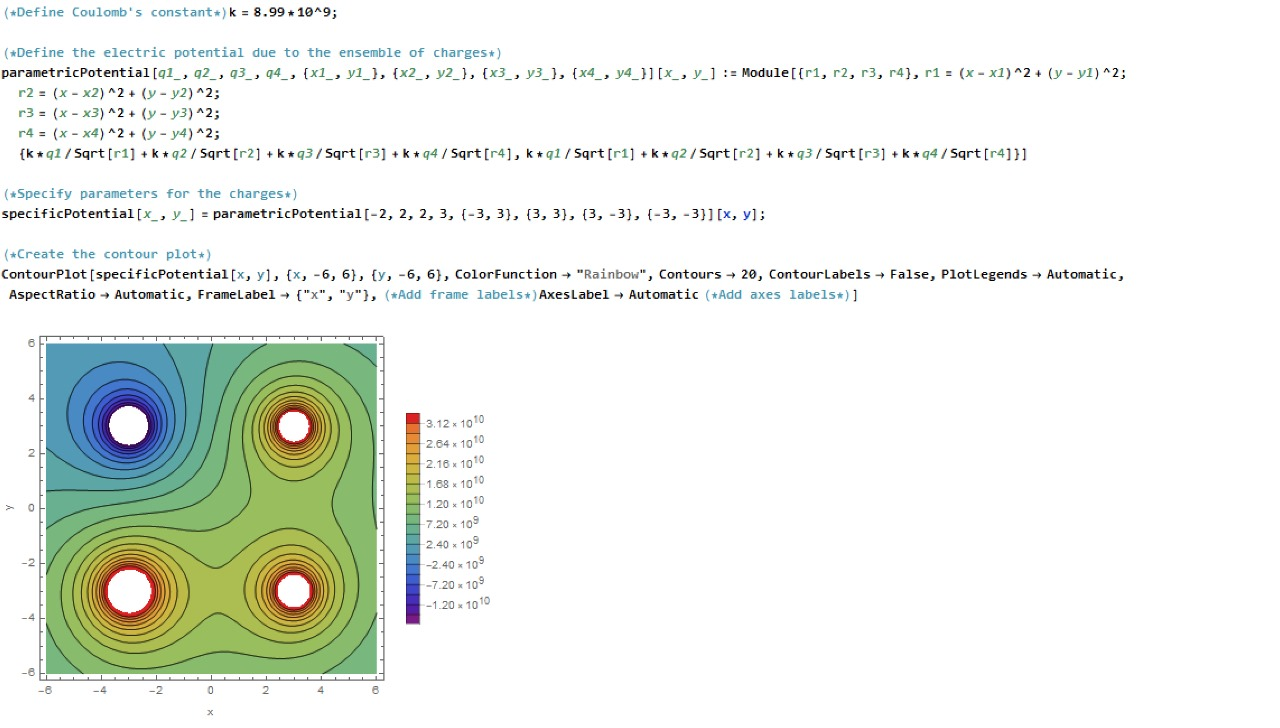
\includegraphics[scale=0.5]{figs/v2.jpeg}
    \caption{}    
    \label{fig:ishitha.em.fig1}
   \end{figure} 
   
   \newpage

(c) \begin{figure}[H]
    \centering
     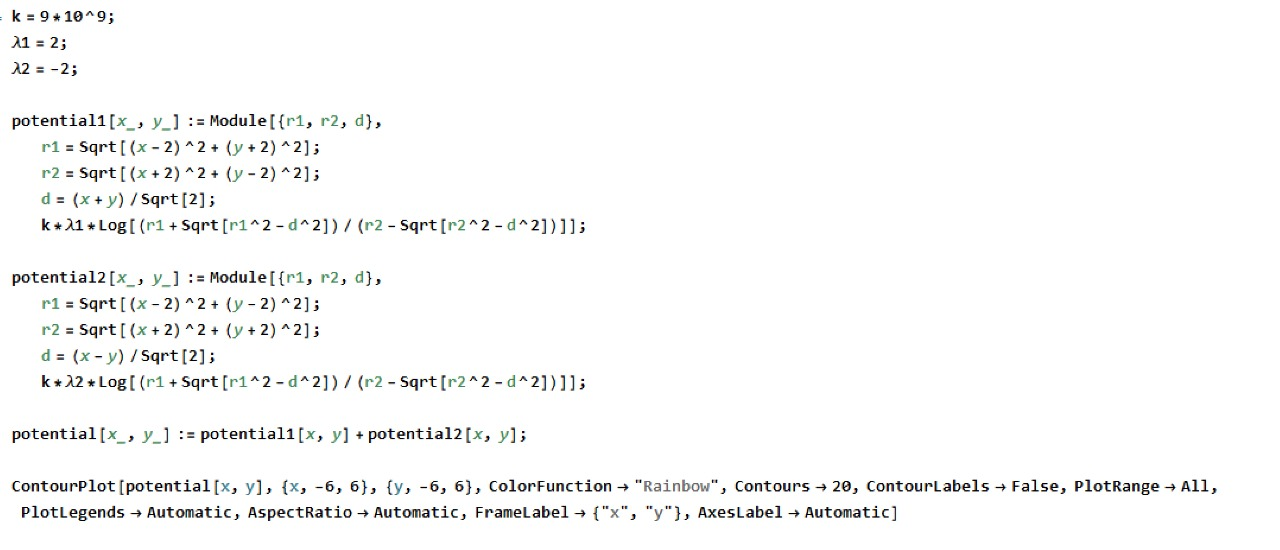
\includegraphics[scale=0.5]{figs/v3.1.jpeg}
    \caption{}    
    \label{fig:ishitha.em.fig1}
   \end{figure}   
   \begin{figure}[H]
    \centering
     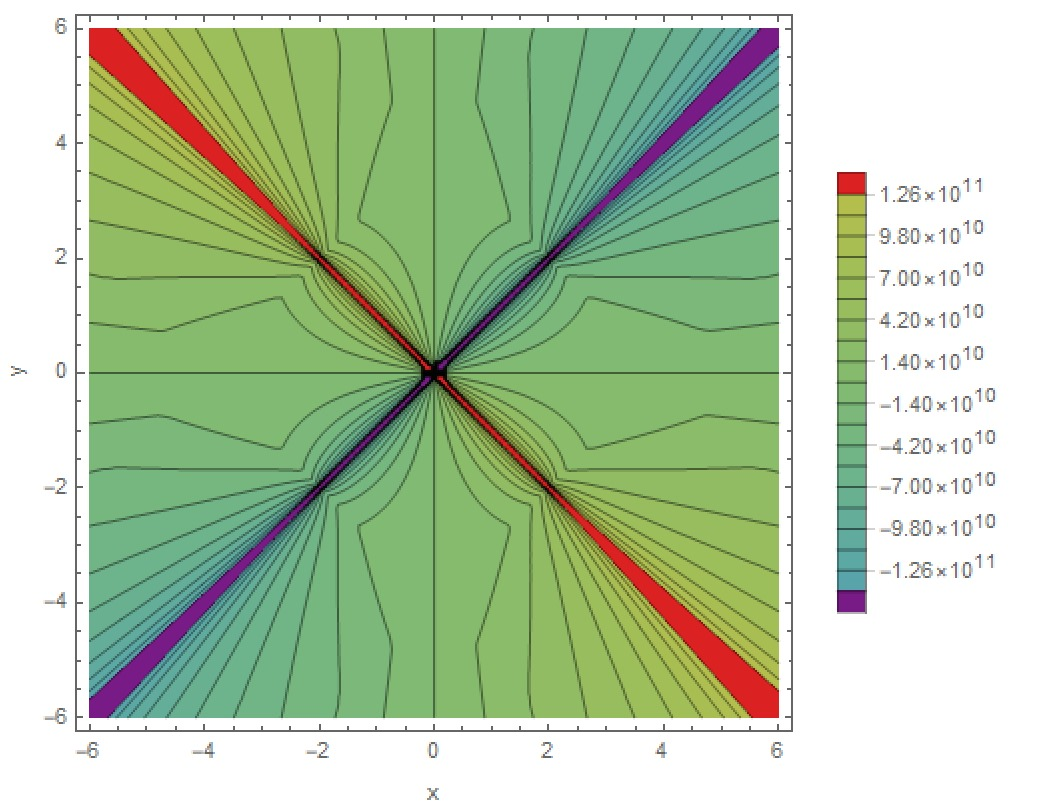
\includegraphics[scale=0.5]{figs/v3.jpeg}
    \caption{}    
    \label{fig:ishitha.em.fig1}
   \end{figure}     

\newpage
(2.1.(c))\\
(a)\begin{figure}[H]
    \centering
     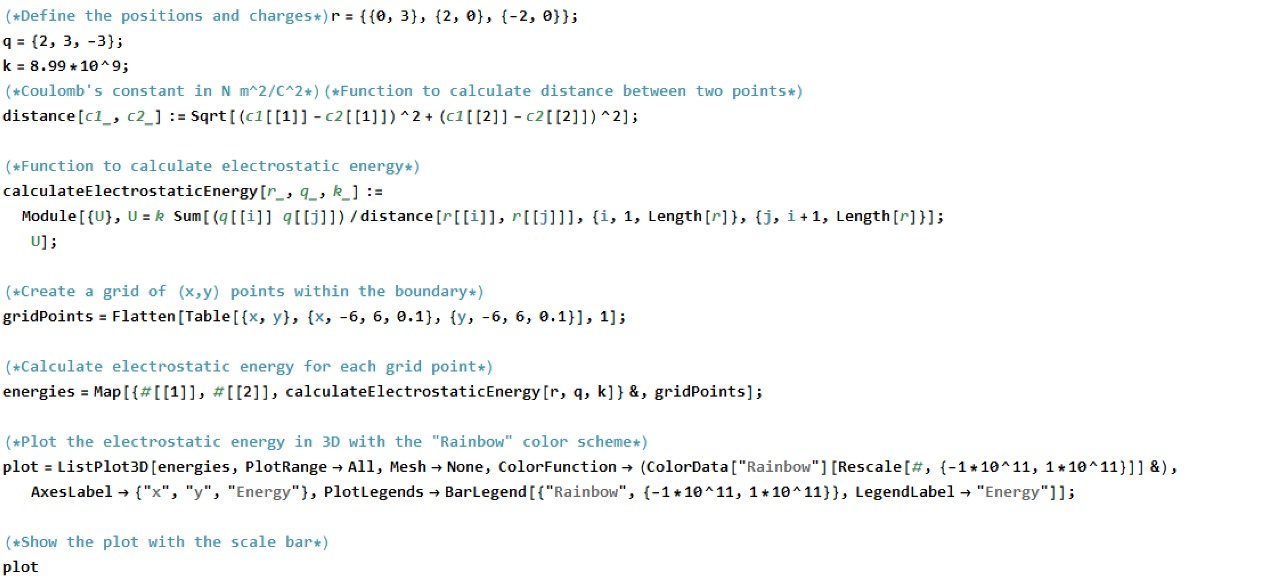
\includegraphics[scale=0.5]{figs/u2.1.a.1.jpeg}
    \caption{}    
    \label{fig:ishitha.em.fig1}
   \end{figure} 
   \begin{figure}[H]
    \centering
     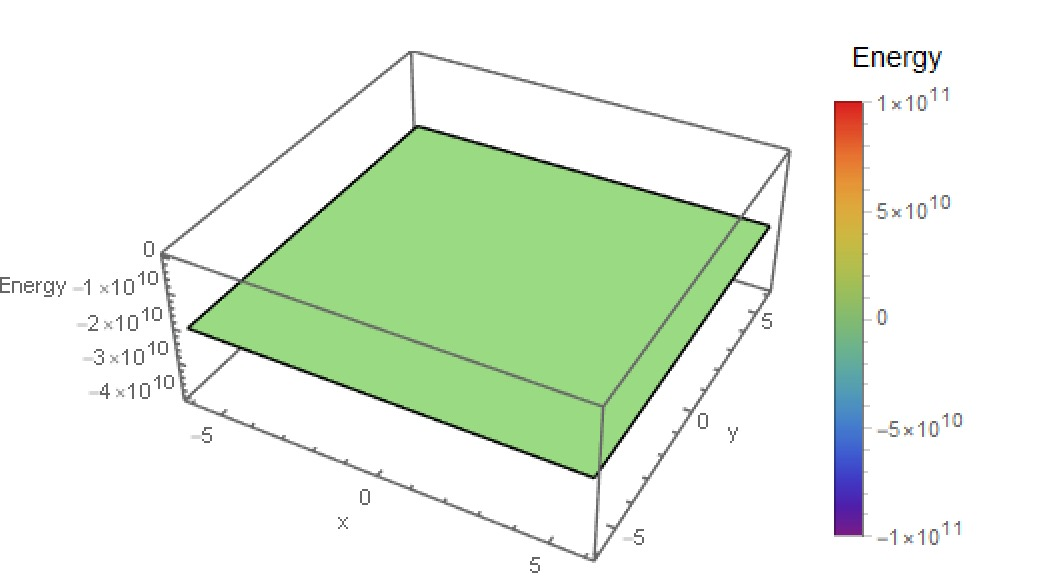
\includegraphics[scale=0.5]{figs/u2.1.a.jpeg}
    \caption{}    
    \label{fig:ishitha.em.fig1}
   \end{figure} 
   
 \newpage
 
(b)   \begin{figure}[H]
    \centering
     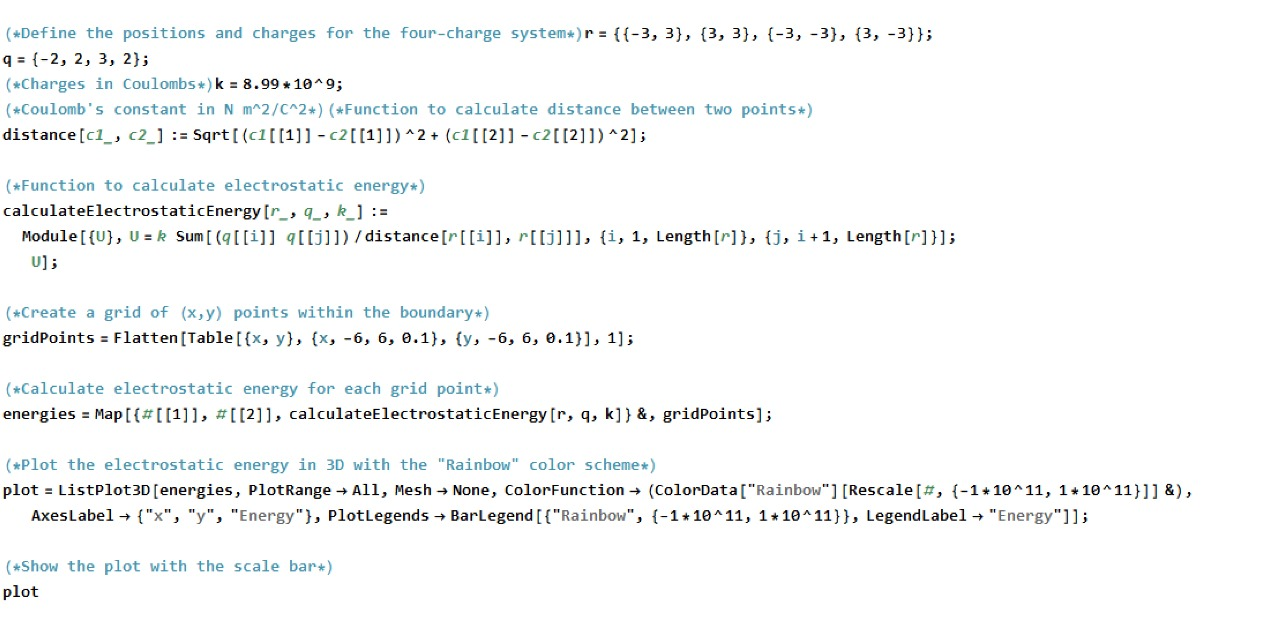
\includegraphics[scale=0.5]{figs/u2.2.b.1.jpeg}
    \caption{}    
    \label{fig:ishitha.em.fig1}
   \end{figure} 
   \begin{figure}[H]
    \centering
     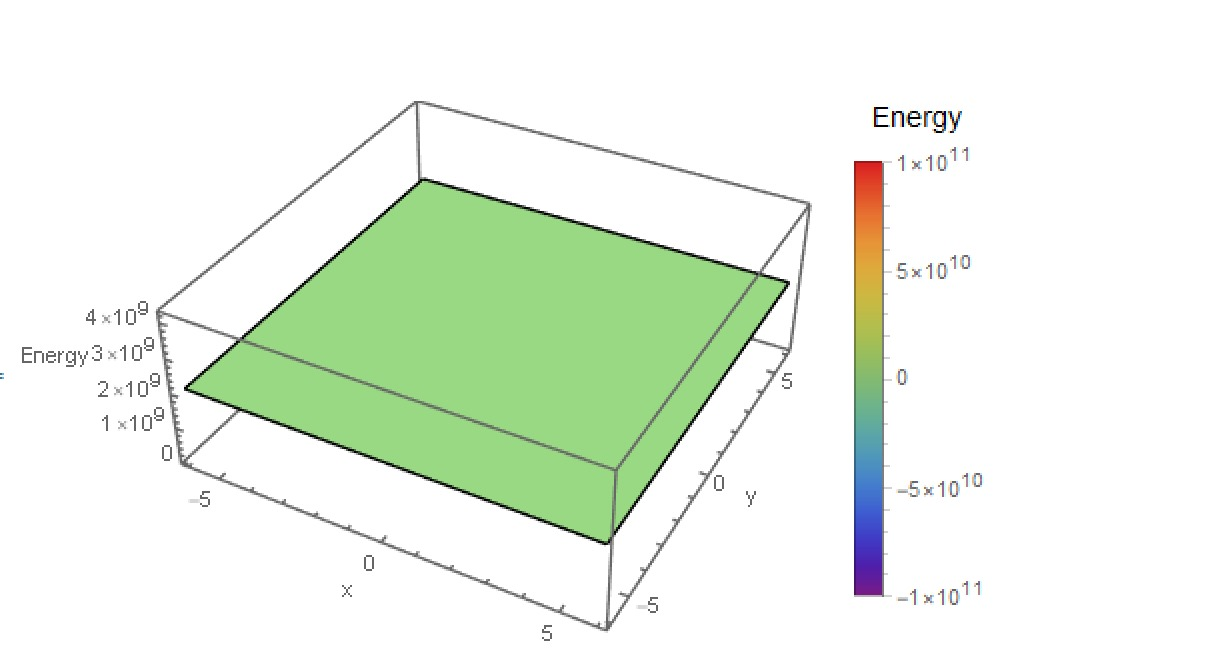
\includegraphics[scale=0.5]{figs/u2.2.b.jpeg}
    \caption{}    
    \label{fig:ishitha.em.fig1}
   \end{figure} 
   
\newpage
(c)\begin{figure}[H]
    \centering
     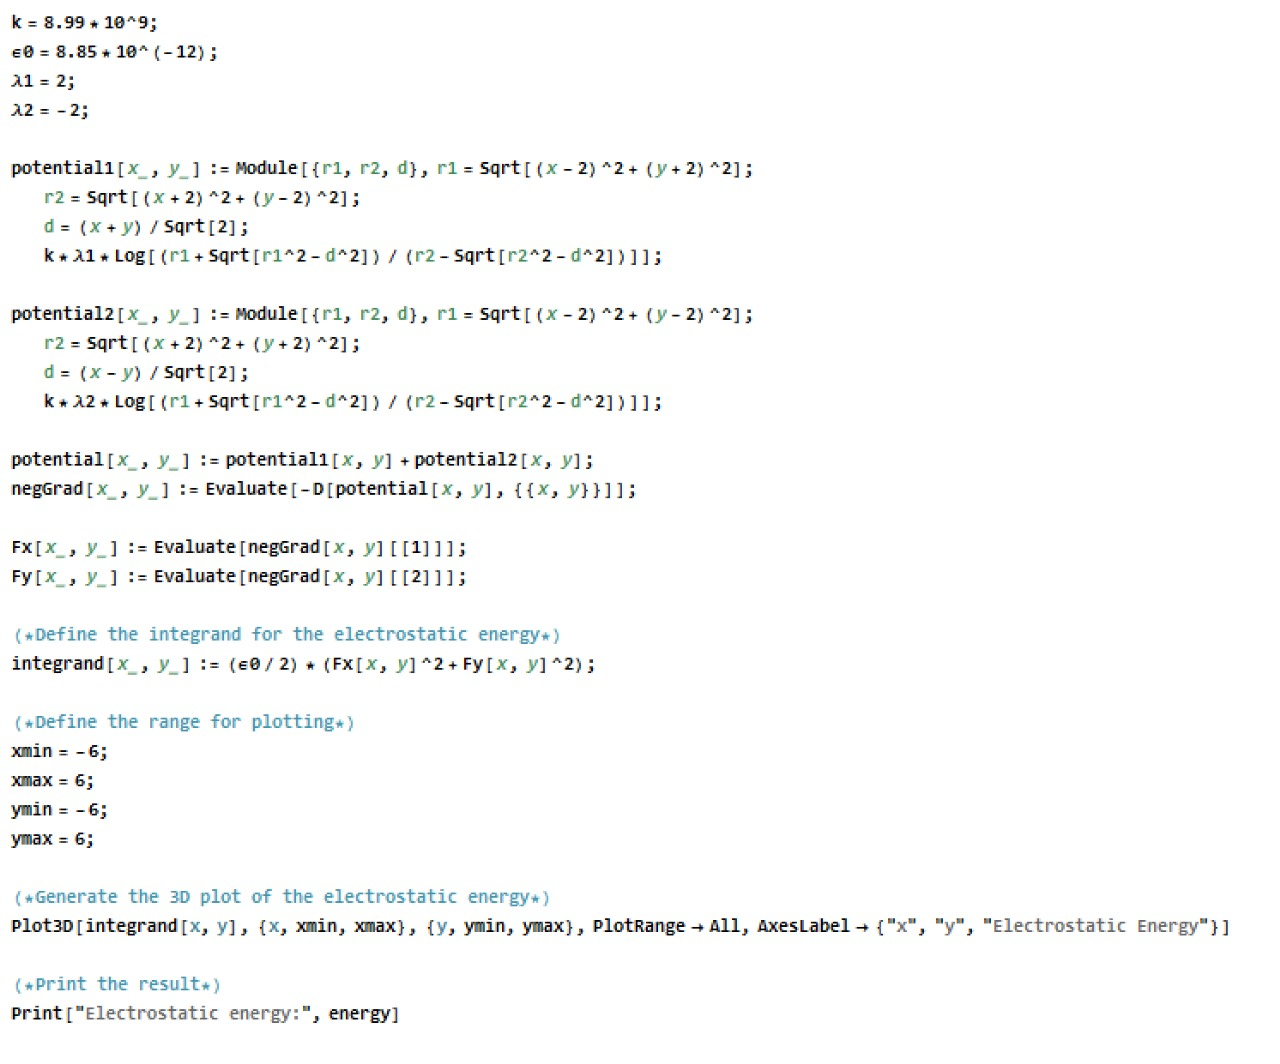
\includegraphics[scale=0.5]{figs/u31.jpeg}
    \caption{}    
    \label{fig:ishitha.em.fig1}
   \end{figure} 
   \begin{figure}[H]
    \centering
     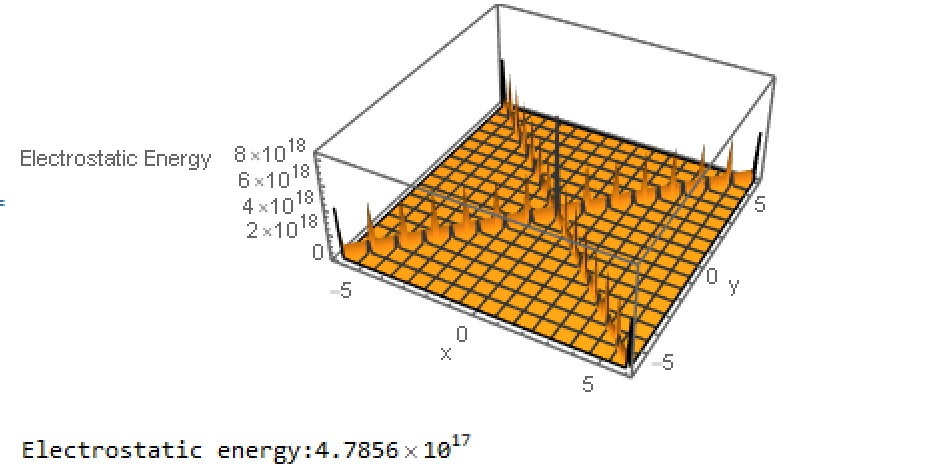
\includegraphics[scale=0.5]{figs/u32.jpeg}
    \caption{}    
    \label{fig:ishitha.em.fig1}
   \end{figure}  

    
(2.2.(a))\\
(2.2.(b))\\
(a)\begin{figure}[H]
    \centering
     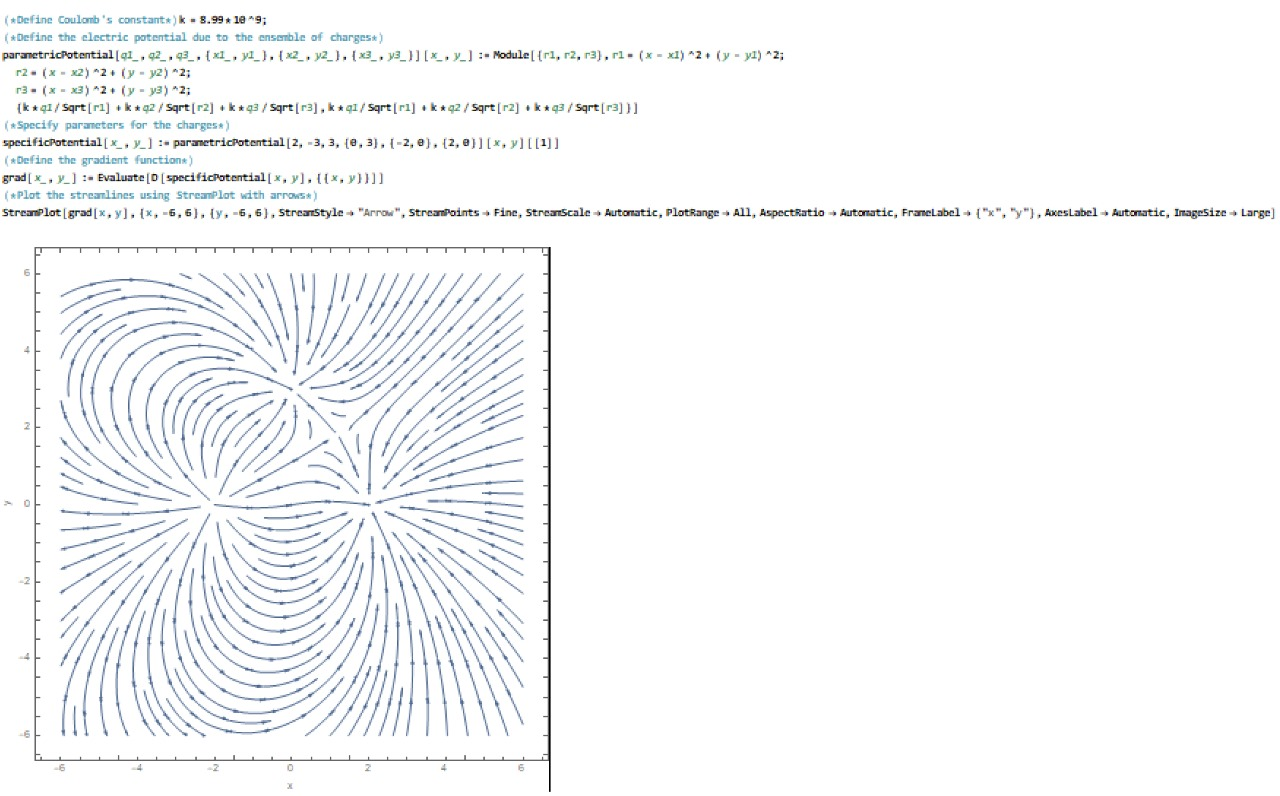
\includegraphics[scale=0.5]{figs/e.3.jpeg}
    \caption{}    
    \label{fig:ishitha.em.fig1}
   \end{figure} 
 hence, $\overrightarrow{E}=-\nabla\overrightarrow{V}  $\\
\newpage 
 (b)\begin{figure}[H]
    \centering
     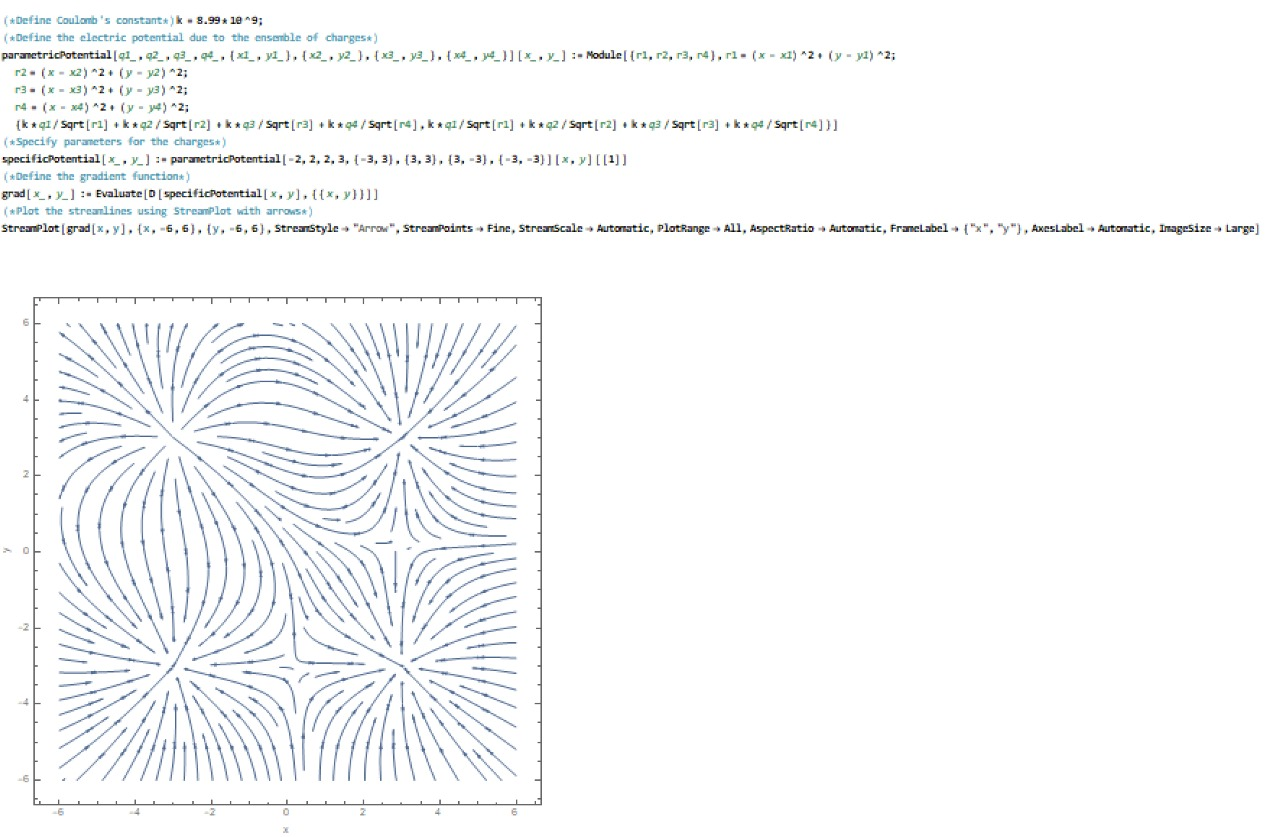
\includegraphics[scale=0.5]{figs/e.2.jpeg}
    \caption{}    
    \label{fig:ishitha.em.fig1}
   \end{figure} 
 hence, $\overrightarrow{E}=-\nabla\overrightarrow{V}  $\\
 (c)\begin{figure}[H]
    \centering
     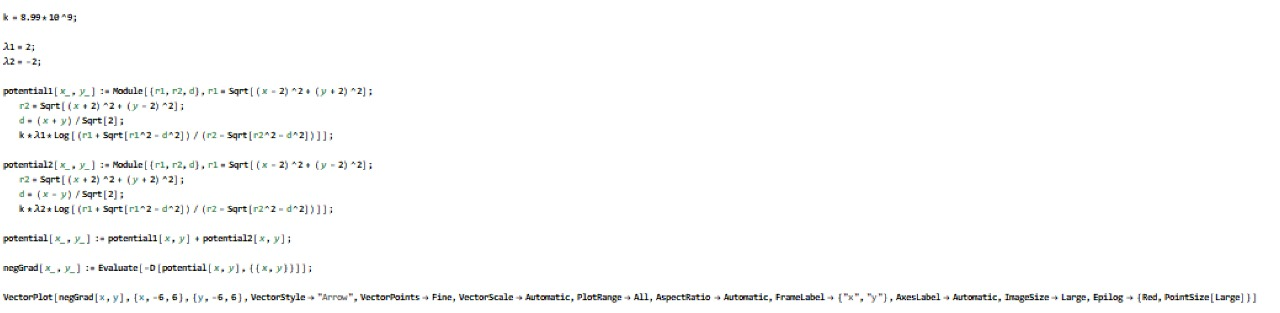
\includegraphics[scale=0.55]{figs/e.1.1.jpeg}
    \caption{}    
    \label{fig:ishitha.em.fig1}
   \end{figure} \begin{figure}[H]
    \centering
     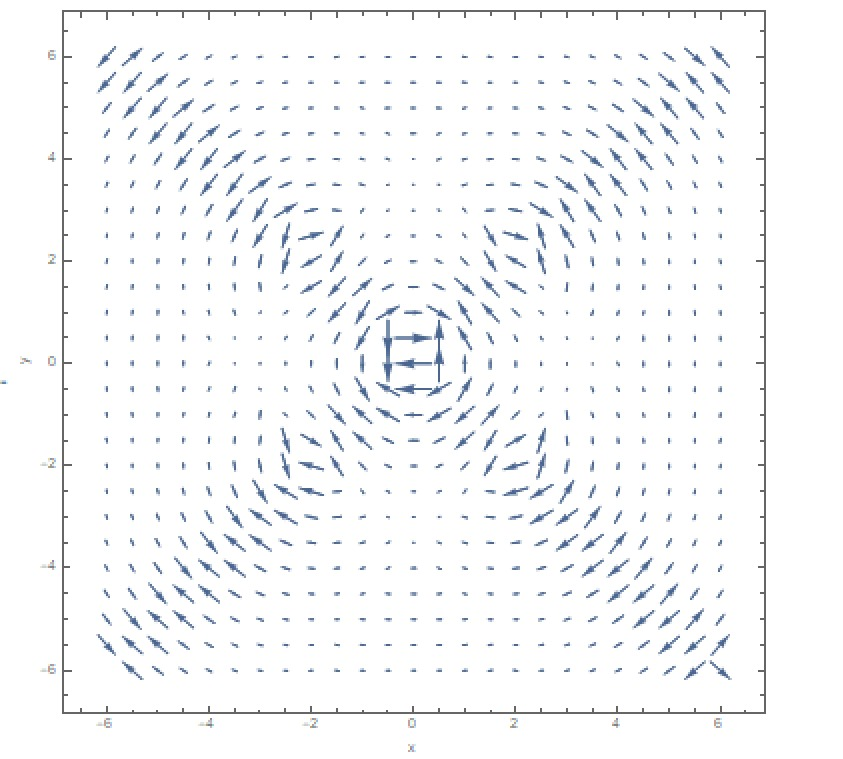
\includegraphics[scale=0.5]{figs/e.1.jpeg}
    \caption{}    
    \label{fig:ishitha.em.fig1}
   \end{figure}
 hence, $\overrightarrow{E}=-\nabla\overrightarrow{V}  $    \\ 
 \newpage
(2.2.(c))\\
(a)
\begin{figure}[H]
    \centering
     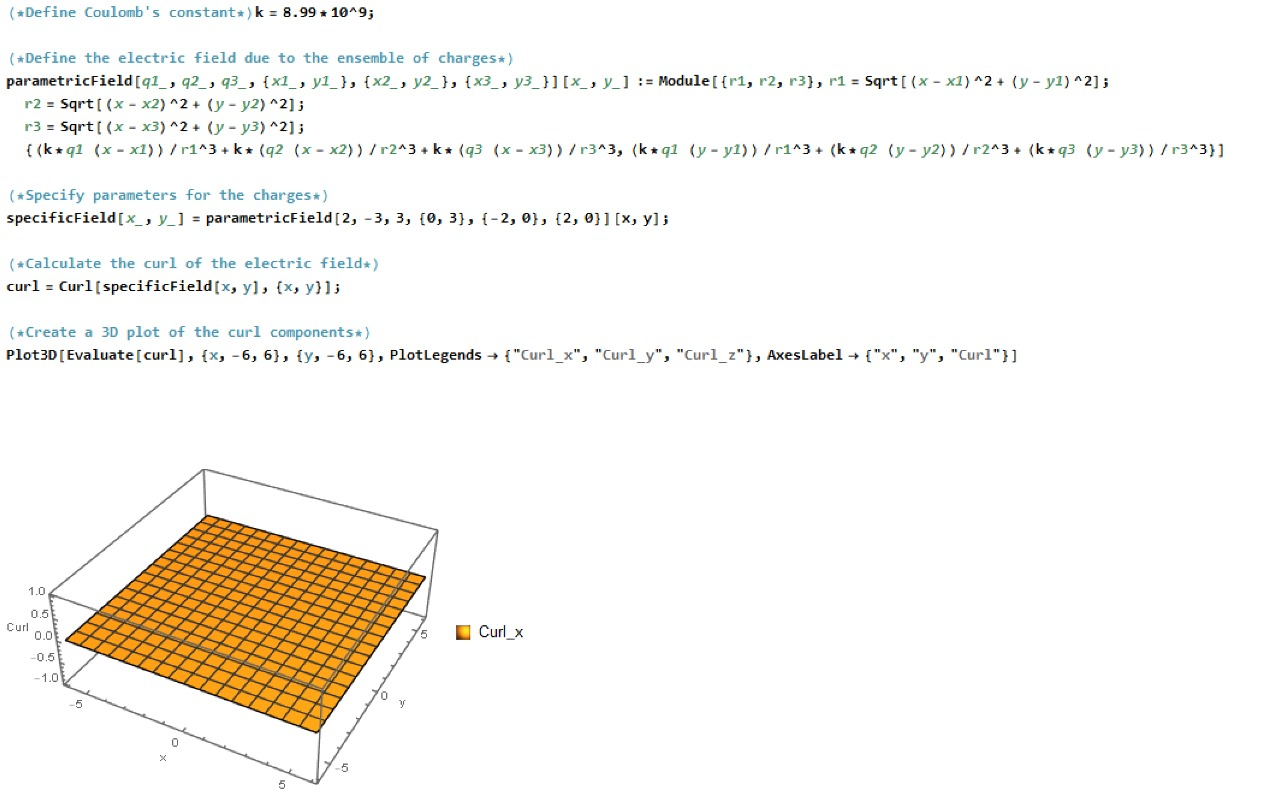
\includegraphics[scale=0.5]{figs/c1.jpeg}
    \caption{}    
    \label{fig:ishitha.em.fig1}
   \end{figure} 
  
(b)   \begin{figure}[H]
    \centering
     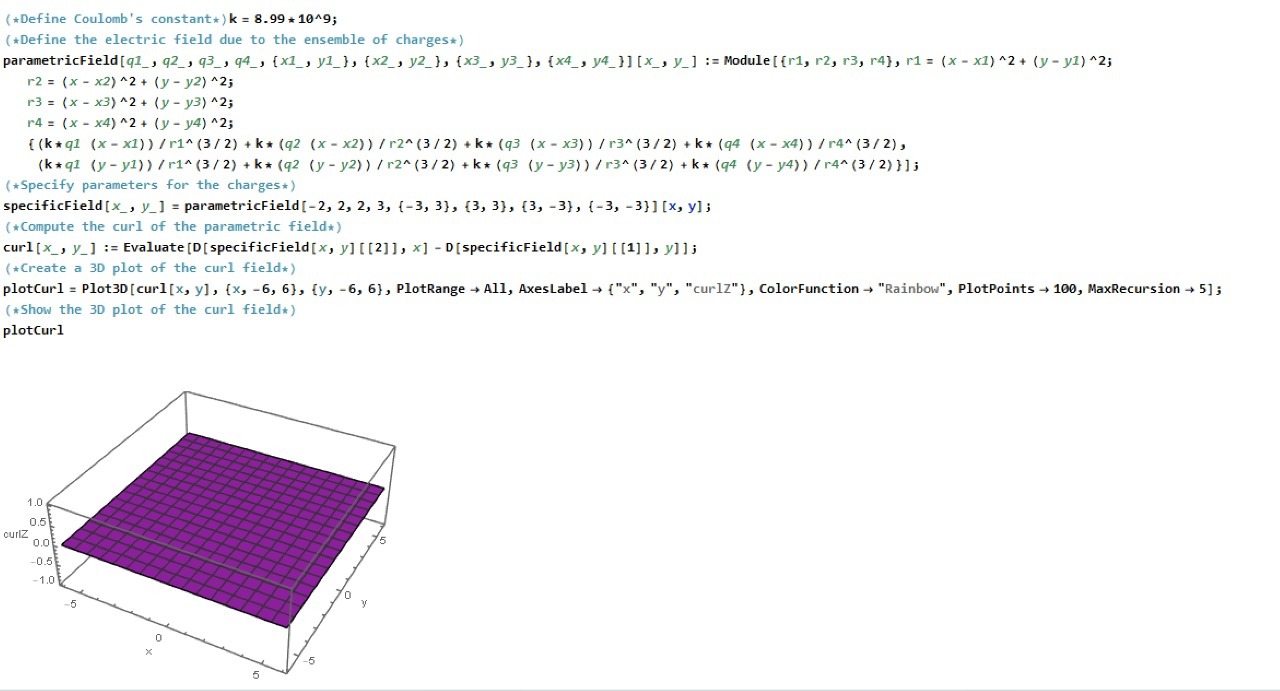
\includegraphics[scale=0.5]{figs/c2.jpeg}
    \caption{}    
    \label{fig:ishitha.em.fig1}
   \end{figure} 
   
(c)  \begin{figure}[H]
    \centering
     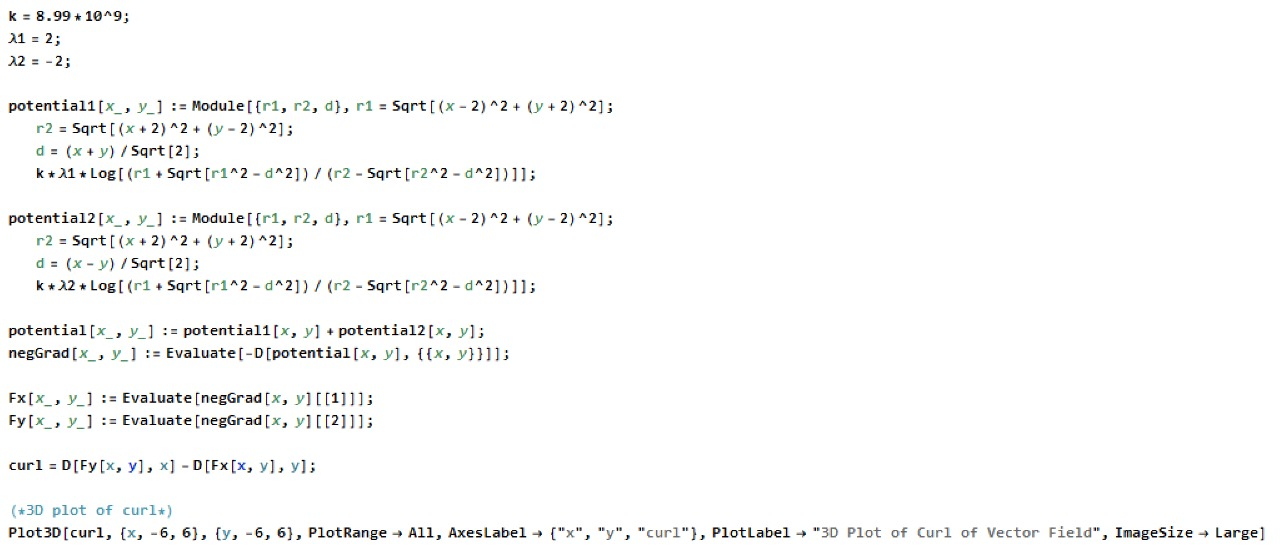
\includegraphics[scale=0.5]{figs/c31.jpeg}
    \caption{}    
    \label{fig:ishitha.em.fig1}
   \end{figure}   
    \begin{figure}[H]
    \centering
     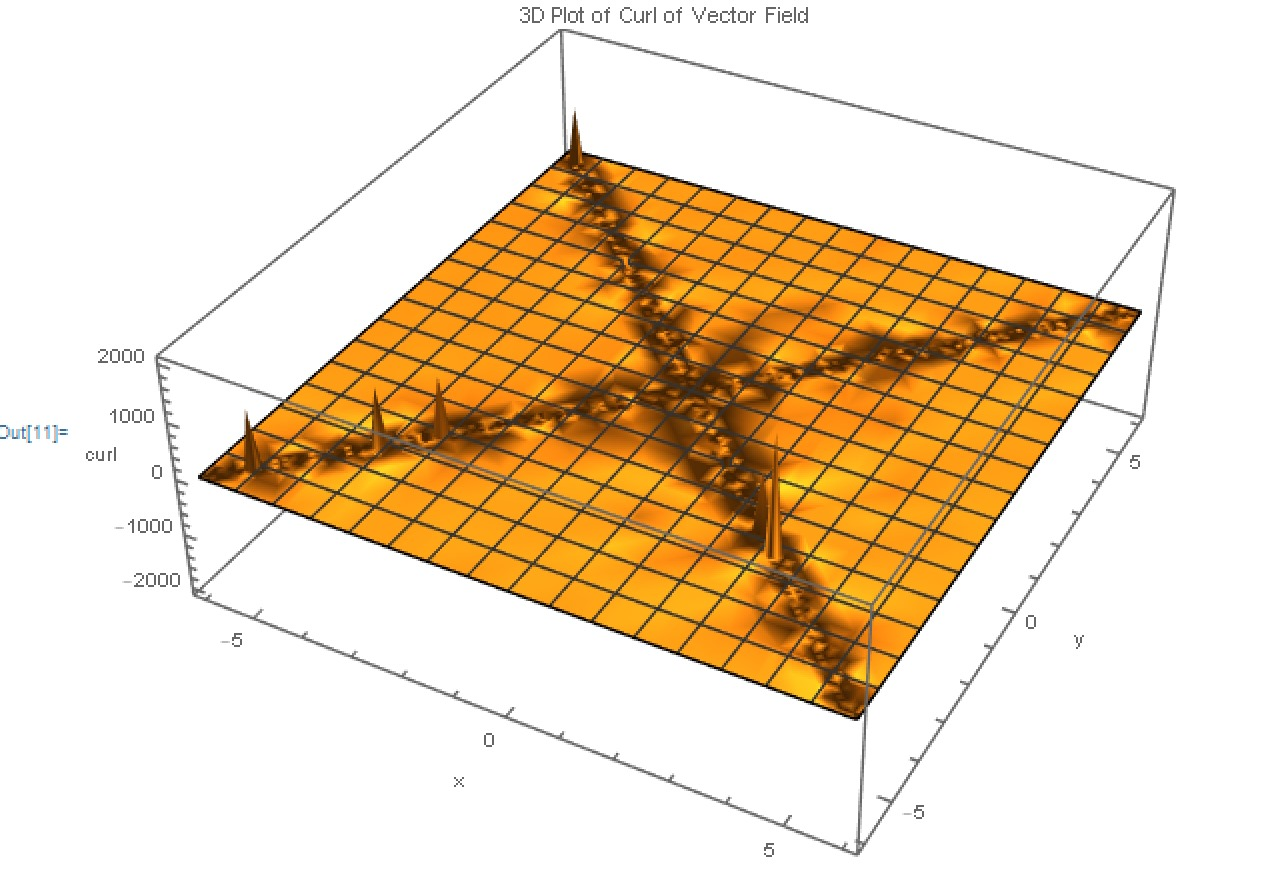
\includegraphics[scale=0.5]{figs/c32.jpeg}
    \caption{}    
    \label{fig:ishitha.em.fig1}
   \end{figure} 
  \newpage    
(2.3)\\
(a)\begin{figure}[H]
    \centering
     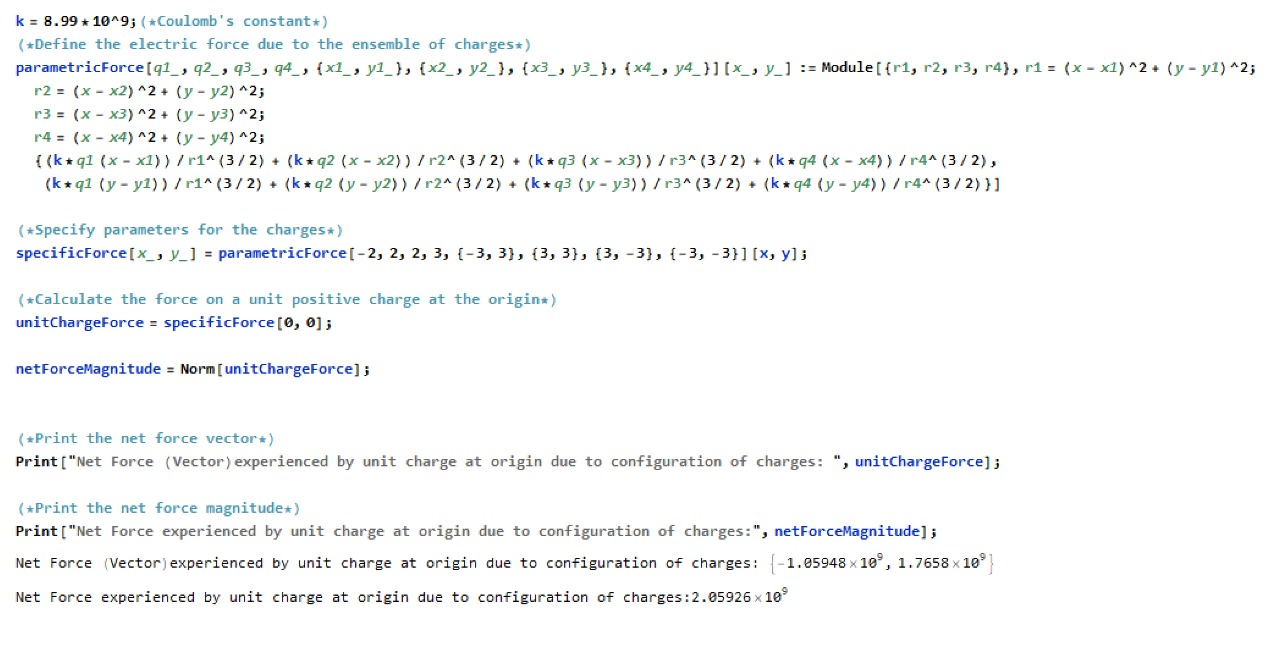
\includegraphics[scale=0.5]{figs/f1.jpeg}
    \caption{}    
    \label{fig:ishitha.em.fig1}
   \end{figure} 
 
(b) \begin{figure}[H]
    \centering
     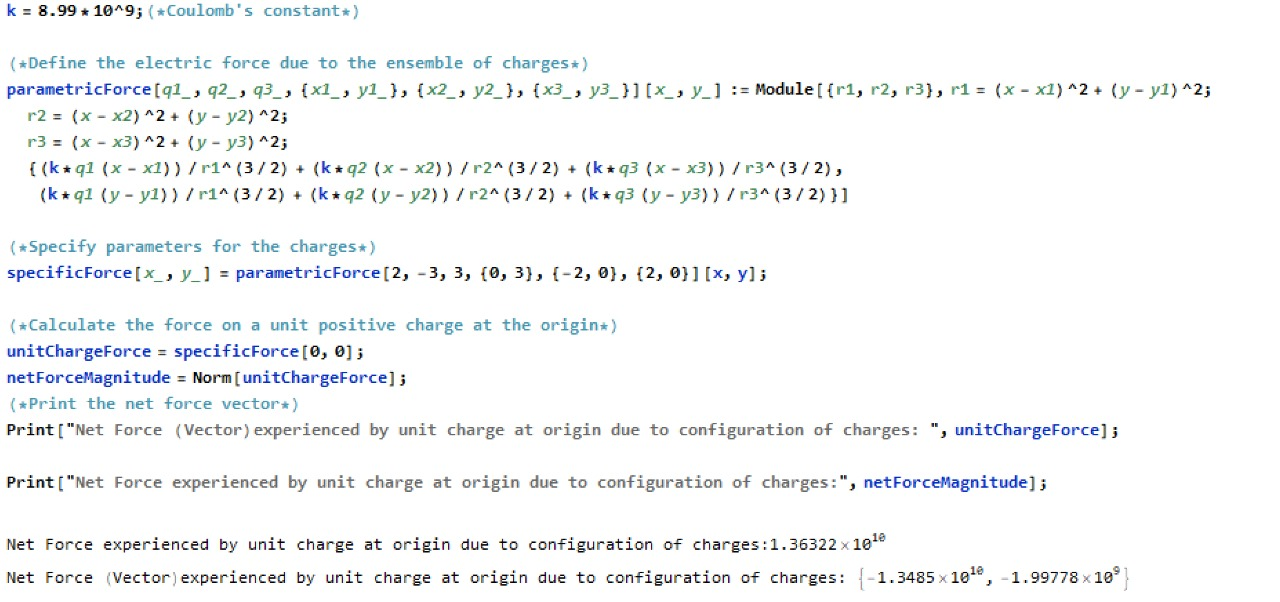
\includegraphics[scale=0.5]{figs/f2.jpeg}
    \caption{}    
    \label{fig:ishitha.em.fig1}
   \end{figure} 
   \newpage   
(c)  \begin{figure}[H]
    \centering
     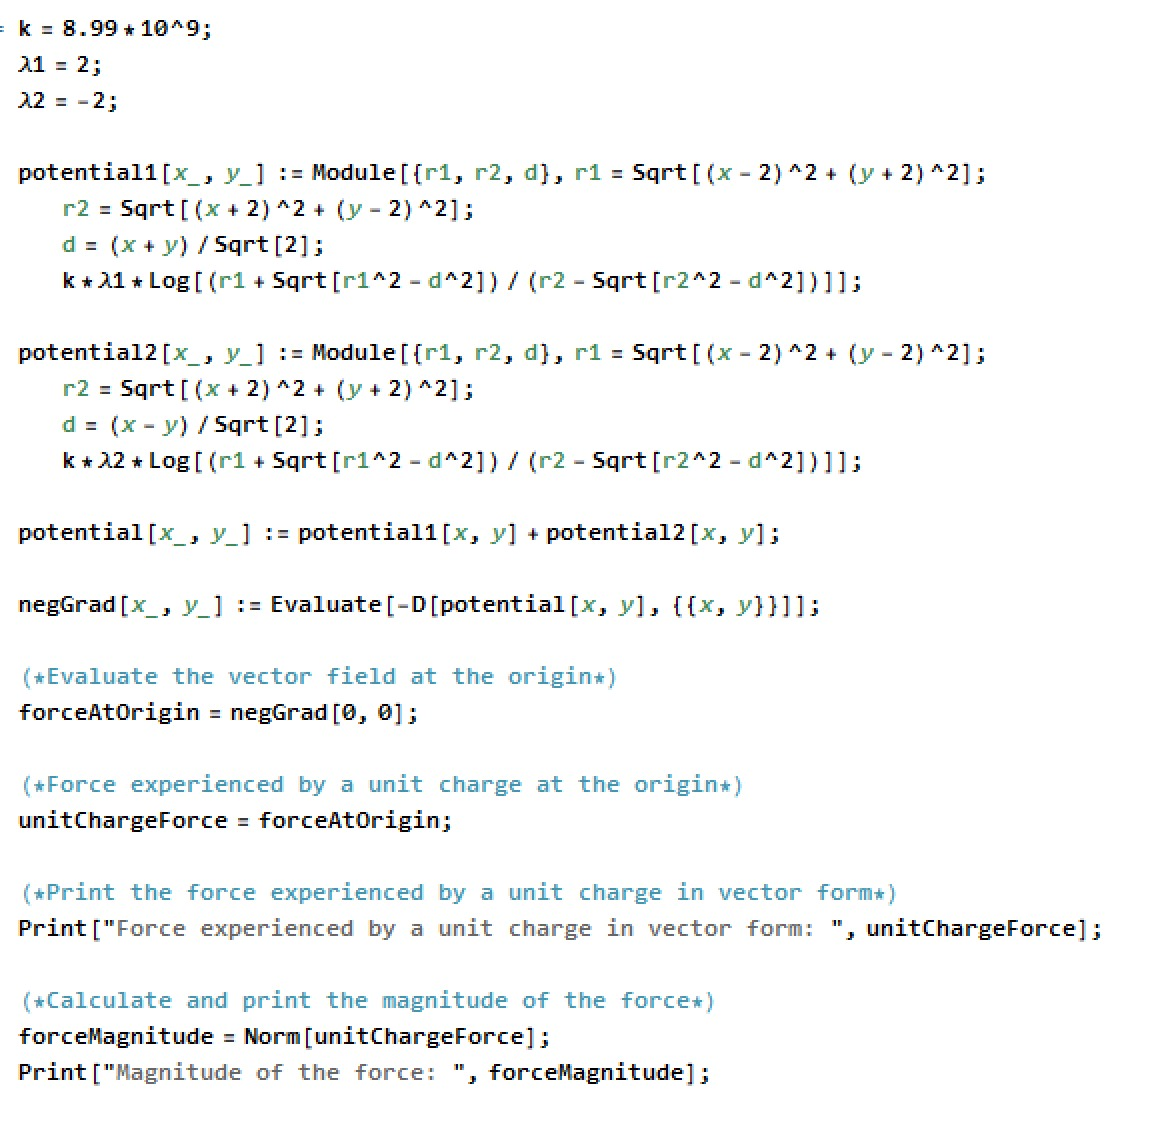
\includegraphics[scale=0.5]{figs/f3.jpeg}
    \caption{}    
    \label{fig:ishitha.em.fig1}
   \end{figure}   
    \begin{figure}[H]
    \centering
     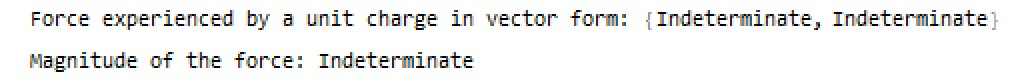
\includegraphics[scale=0.5]{figs/f3o.jpeg}
    \caption{}    
    \label{fig:ishitha.em.fig1}
   \end{figure}    
   
3: Simulating fields and potential on a simulator \\
(a) Select any open source/institute licensed electromagnetics simulator. \\
(b) Draw a 2-D geometry comprising metal/insulator , semiconductor is optional. Explain the significance/ why you chose this geometry.$[3 points]$ \\
(c) Select/choose the correct equations $\&$\ boundary conditions and justify them.$[2 points]$ \\
(d) Plot/Represent the $\overrightarrow{E}$ $\&$ V fields,what svientific sights you gain out of this?$[5 points]$\\

\solution
The electromagnetic simulator we are using is \textit{sim scale}, which is open source.\\
 
The geometry we are using is \textbf{circular plate}.\\

\textbf{We are choosing a circular plate for the following reasons:}

\begin{itemize}
  \item The metal plate acts as a conductor and the surrounding medium (air) acts as an insulator. The geometry is very simple and allows the study of the behavior of electric fields and electric potential.
  \item The circular plate has more symmetry and a uniform field distribution.
  \item The circular geometry provides simple analytical solutions compared to other complex geometries. 
  \item In our regular life, the circular structures are used in many practical appliances. so studying this geometry gives insights to other real world devices.
\end{itemize}

\textbf{The boundary conditions for the circular plate are:}

\begin{enumerate}
  \item The boundary condition for the electric field is that the tangential part of the electric field must be zero so that the electric field lines will be perpendicular to the surface of the conductor, making it an ideal conductor:
  \[ E_t = 0 \]

  \item The boundary condition for the electrostatic potential is that the gradient of the electrostatic potential normal to the surface should be zero, ensuring that the electrostatic potential is constant throughout:
  \[ \frac{\partial V}{\partial n} = 0 \]
\end{enumerate}

where, \( n \) is the normal vector pointing outwards from the surface.


\end{document}
